%%%%%%%%%%%%%%%%%%%%%%%%%%%%%%%%%%%%%%%%%
% Wenneker Article
% LaTeX Template
% Version 2.0 (28/2/17)
%
% This template was downloaded from:
% http://www.LaTeXTemplates.com
%
% Authors:
% Vel (vel@LaTeXTemplates.com)
% Frits Wenneker
%
% License:
% CC BY-NC-SA 3.0 (http://creativecommons.org/licenses/by-nc-sa/3.0/)
%
%%%%%%%%%%%%%%%%%%%%%%%%%%%%%%%%%%%%%%%%%

%----------------------------------------------------------------------------------------
%	PACKAGES AND OTHER DOCUMENT CONFIGURATIONS
%----------------------------------------------------------------------------------------

\documentclass[12pt, a4paper]{article} % 10pt font size (11 and 12 also possible), A4 paper (letterpaper for US letter) and two column layout (remove for one column)

%%%%%%%%%%%%%%%%%%%%%%%%%%%%%%%%%%%%%%%%%
% Wenneker Article
% Structure Specification File
% Version 1.0 (28/2/17)
%
% This file originates from:
% http://www.LaTeXTemplates.com
%
% Authors:
% Frits Wenneker
% Vel (vel@LaTeXTemplates.com)
%
% License:
% CC BY-NC-SA 3.0 (http://creativecommons.org/licenses/by-nc-sa/3.0/)
%
%%%%%%%%%%%%%%%%%%%%%%%%%%%%%%%%%%%%%%%%%

%----------------------------------------------------------------------------------------
%	PACKAGES AND OTHER DOCUMENT CONFIGURATIONS
%----------------------------------------------------------------------------------------

\usepackage[english]{babel} % English language hyphenation

\usepackage{setspace}

\usepackage{microtype} % Better typography

\usepackage{amsmath,amsfonts,amsthm} % Math packages for equations

\usepackage[svgnames]{xcolor} % Enabling colors by their 'svgnames'

\usepackage[hang, small, labelfont=bf, up, textfont=it]{caption} % Custom captions under/above tables and figures

\usepackage{booktabs} % Horizontal rules in tables

\usepackage{lastpage} % Used to determine the number of pages in the document (for "Page X of Total")

\usepackage{graphicx} % Required for adding images
\graphicspath{ {./images/} }
\usepackage{subfig}

\usepackage{enumitem} % Required for customising lists
\setlist{noitemsep} % Remove spacing between bullet/numbered list elements

\usepackage{sectsty} % Enables custom section titles
\allsectionsfont{\usefont{OT1}{phv}{b}{n}} % Change the font of all section commands (Helvetica)

%----------------------------------------------------------------------------------------
%	MARGINS AND SPACING
%----------------------------------------------------------------------------------------

\usepackage{geometry} % Required for adjusting page dimensions

\geometry{
	top=1cm, % Top margin
	bottom=1.5cm, % Bottom margin
	left=2cm, % Left margin
	right=2cm, % Right margin
	includehead, % Include space for a header
	includefoot, % Include space for a footer
	%showframe, % Uncomment to show how the type block is set on the page
}

\setlength{\columnsep}{7mm} % Column separation width

%----------------------------------------------------------------------------------------
%	FONTS
%----------------------------------------------------------------------------------------

\usepackage[T1]{fontenc} % Output font encoding for international characters
\usepackage[utf8]{inputenc} % Required for inputting international characters

\usepackage{XCharter} % Use the XCharter font

%----------------------------------------------------------------------------------------
%	HEADERS AND FOOTERS
%----------------------------------------------------------------------------------------

\usepackage{fancyhdr} % Needed to define custom headers/footers
\pagestyle{fancy} % Enables the custom headers/footers

\renewcommand{\headrulewidth}{0.0pt} % No header rule
\renewcommand{\footrulewidth}{0.4pt} % Thin footer rule

\renewcommand{\sectionmark}[1]{\markboth{#1}{}} % Removes the section number from the header when \leftmark is used

%\nouppercase\leftmark % Add this to one of the lines below if you want a section title in the header/footer

% Headers
\lhead{} % Left header
\chead{\textit{\thetitle}} % Center header - currently printing the article title
\rhead{} % Right header

% Footers
\lfoot{} % Left footer
\cfoot{} % Center footer
\rfoot{\footnotesize Page \thepage\ of \pageref{LastPage}} % Right footer, "Page 1 of 2"

\fancypagestyle{firstpage}{ % Page style for the first page with the title
	\fancyhf{}
	\renewcommand{\footrulewidth}{0pt} % Suppress footer rule
}

%----------------------------------------------------------------------------------------
%	TITLE SECTION
%----------------------------------------------------------------------------------------

\newcommand{\authorstyle}[1]{{\large\usefont{OT1}{phv}{b}{n}\color{DarkRed}#1}} % Authors style (Helvetica)

\newcommand{\institution}[1]{{\footnotesize\usefont{OT1}{phv}{m}{sl}\color{Black}#1}} % Institutions style (Helvetica)

\usepackage{titling} % Allows custom title configuration

\newcommand{\HorRule}{\color{DarkGoldenrod}\rule{\linewidth}{1pt}} % Defines the gold horizontal rule around the title

\pretitle{
	\vspace{-30pt} % Move the entire title section up
	\HorRule\vspace{10pt} % Horizontal rule before the title
	\fontsize{24}{28}\usefont{OT1}{phv}{b}{n}\selectfont % Helvetica
	\color{DarkRed} % Text colour for the title and author(s)
}

\posttitle{\par\vskip 10pt} % Whitespace under the title

\preauthor{} % Anything that will appear before \author is printed

\postauthor{ % Anything that will appear after \author is printed
	\vspace{10pt} % Space before the rule
	\par\HorRule % Horizontal rule after the title
	\vspace{20pt} % Space after the title section
}

%----------------------------------------------------------------------------------------
%	ABSTRACT
%----------------------------------------------------------------------------------------

\usepackage{lettrine} % Package to accentuate the first letter of the text (lettrine)
\usepackage{fix-cm}	% Fixes the height of the lettrine

\newcommand{\initial}[1]{ % Defines the command and style for the lettrine
	\lettrine[lines=3,findent=4pt,nindent=0pt]{% Lettrine takes up 3 lines, the text to the right of it is indented 4pt and further indenting of lines 2+ is stopped
		\color{DarkGoldenrod}% Lettrine colour
		{#1}% The letter
	}{}%
}

\usepackage{xstring} % Required for string manipulation

\newcommand{\lettrineabstract}[1]{
	\StrLeft{#1}{1}[\firstletter] % Capture the first letter of the abstract for the lettrine
	\initial{\firstletter}\textbf{\StrGobbleLeft{#1}{1}} % Print the abstract with the first letter as a lettrine and the rest in bold
}

%----------------------------------------------------------------------------------------
%	BIBLIOGRAPHY
%----------------------------------------------------------------------------------------

\usepackage[backend=bibtex,style=authoryear,natbib=true]{biblatex} % Use the bibtex backend with the authoryear citation style (which resembles APA)

\addbibresource{example.bib} % The filename of the bibliography

\usepackage[autostyle=true]{csquotes} % Required to generate language-dependent quotes in the bibliography
 % Specifies the document structure and loads requires packages

%----------------------------------------------------------------------------------------
%	ARTICLE INFORMATION
%----------------------------------------------------------------------------------------

\title{Supervised Classification of Monte Carlo Simulated Air Shower Data} % The article title

\author{
	\authorstyle{Jeffrey Tumminia} % Authors
}

% Example of a one line author/institution relationship
%\author{\newauthor{John Marston} \newinstitution{Universidad Nacional Autónoma de México, Mexico City, Mexico}}


%----------------------------------------------------------------------------------------
\doublespacing

\date{}
  
\begin{document}

\maketitle % Print the title

\thispagestyle{firstpage} % Apply the page style for the first page (no headers and footers)

%----------------------------------------------------------------------------------------
%	ABSTRACT
%----------------------------------------------------------------------------------------

\abstract{As we probe nature for more fundamental theories of reality, we find that experimentation is yielding larger and noisier datasets \citep{PETA}. This leads to calls for effective data science techniques in projects such as the MAGIC (Major Atmospheric Gamma Imaging Cherenkov) Telescope, a ground based high energy electromagnetic wave detector \citep{MAGIC}. One application of MAGIC is to observe high energy EM air showers caused by $\gamma$-rays, where $\gamma$-ray observation is usually done by much more costly satellite/balloon based telescopes \citep{energyCRs}. We generate multiple Supervised Learning models, tuned selected models and build a hard Voting Classifier to classify these air showers. All models are trained,validated and tested using the MAGIC dataset $M$, generated using a Monte Carlo Air shower Simulation tool called CORSIKA \citep{DataProd}. $M$ is a collection 19020 air showers classified as the result of a $\gamma$-ray or hadronic shower which is expected to be challenging for linear classification, and we follow protocol and benchmarks outlined in the by the developers of $M$ \citep{CaseStudy} }

%----------------------------------------------------------------------------------------
%	ARTICLE CONTENTS
%----------------------------------------------------------------------------------------

\newpage
\section{Business and Data Understanding}

\subsection{Background of $\gamma$-Rays}

$\gamma$ rays were first identified as waves in the electromagnetic (EM) spectrum in the early 1900's by Ernest Rutherford \citep{Ruth}. Since the discovery, physicists have been trying to develop tools to detect $\gamma$-rays and their properties. Explorer XI was launched by NASA in 1961, and was the first telescope dedicated to $\gamma$-ray detection, which detected a total of 22 $\gamma$-ray events in it's lifetime. Since then, technology has progressed and we have continued to put up larger and more accurate detectors, allowing us to map our galaxy in $\gamma$-rays and detect the emission of $\gamma$-rays from astrological events far out into the universe, giving us a proxy to analyze them. 

Though these telescopes are absolutely amazing in their own right, they have all had at least one major drawback to them, being that they must reside well outside of our atmosphere to function. For instance, the International Gamma-Ray Astrophysics Laboratory (INTEGRAL), which was launched in 2002, reaches a maximum distance above the earths surface of about 150,000km, where as the International Space Station reaches (on average) about 400km. This means that once our $\gamma$-ray telescopes are launched into their orbit, we can never service them again. This has been one of the main bottlenecks limiting what research can be performed, as these incredible telescopes can deplete their energy source or be thrown off of their intended orbit, possibly rendering them useless. This is costly, not only from the perspective of spending resources, but also in the amount of space debris build up this leads to over time. In a time where funding for scientific research is growing thinner with respect to the amount needed to continue progress, there arises a clear motivation to find a better solution for observing characteristics of $\gamma$-rays, if possible.

\subsection{$\gamma$-Ray Detection}

This leads us to the MAGIC (Major Atmospheric Gamma Imaging Cherenkov) Telescope, a ground based high energy electromagnetic wave detector \citep{MAGIC}. One of the goals of MAGIC is to be able to identify $\gamma$-rays that hit earth from the surface and analyze their properties, similar to the satellite based telescopes. In practice, however, this is extremely difficult. 

A primary reason $\gamma$-rays are so difficult to identify from earth is due to our ozone layer, which filters out shorter EM wavelengths (like $\gamma$-rays and X-rays), which would be harmful to life on earth. This does eliminate any course for \textit{direct} detection. However, for very high energy cosmic rays, there is another phenomena we could use as a proxy for identifying them called Cherenkov Radiation. Cherenkov Radiation is usually described as akin to the sonic boom effect but for subatomic particles, where a charged particle is actually traveling faster in a given medium (such as our atmosphere) than a photon would typically travel at in that medium \citep{CherenkovRad}. Note, nothing asserts anything is traveling faster than the speed of light in a vacuum ($c$) in this phenomena. When a cosmic ray hit our upper atmosphere, it collides with atoms (specifically their nuclei) and cause air showers, which caused charged particles to rain down onto the earth's surface. For sufficiently high energy cosmic rays, these charged particles can emit Cherenkov Radiation, which MAGIC (and other ground-based telescopes out of our scope) can detect. This is our detection mechanic.

The major challenge of this method, however, is that $\gamma$-rays are not the only cosmic rays which cause Cherenkov Radiation. Another example of this are hadronic (further referred to as $h$) rays, which are much more common and produce showers with similar features. Furthermore, there is random variance in the patterns of the showers since our atmosphere is not perfectly uniform, thus variance in the characteristics of events of the same class is expected. 

\subsection{Detection as a Classification Problem}

This yields a difficult classification problem, where there is no obvious feature or set of features such that we can easily discriminate results of showers from $\gamma$-rays from $h$-rays. This has led to a wide variety of research in the field attempting to find a mechanism to classify these events. A popular tool for performing this research is CORSIKA: A Monte Carlo Code to Simulate Extensive Air Showers \citep{DataProd}. Using CORSIKA, researchers can simulate air shower events based on numerous parameters which develop a classified dataset which we can then model off of. If one could build an adequate model on the developed dataset, it could be utilized on incoming observations to classify events in real time. It could also possibly identify unusual events that are of interest to researchers. CORSIKA is extremely versatile and could offer a framework for other Monte Carlo Simulation of physical phenomena as well, but that is out of scope. 


One example of this dataset generation is the MAGIC Gamma Telescope Data Set (further referred to as $M$), done by Bock \citep{CaseStudy} and publicly available on the UCI Machine Learning Repository. \cite{CaseStudy} will be heavily referenced going forward, as they perform introductory analysis on the dataset, discuss the dataset limitations, and set performance thresholds for models. We analyze $M$, perform feature engineering and resampling, and train multiple models under varying hyper parameters and build a Voting Classifier in efforts to adequately classify events of $\gamma$-ray air showers based on this dataset. Below are some characteristics noted in the documentation of $M$ and verified in our analysis to remain mindful of throughout this research. 

\begin{itemize}
	\item $M$ contains no missing values
	\item All Features are real numbers
	\item Number of $\gamma$-ray events $>>$ Number of $h$-ray events (purposely)
	\item $dim \left( M \right) = n \times m, n=19020, m=11 \rightarrow n>>m$
\end{itemize}

We also note for our model analysis and scoring that we are much more adverse to false positives than false negatives, as is the case for identifying most phenomena in natural sciences. From this, we declare that our primary model evaluation metrics will be the AUC and precision of the model, though we will keep in mind our recall. These restrictions are also acknowledged in \citep{CaseStudy}. Crucially, when evaluating models which return a probability, we denote that the model should predict an event is a $\gamma$ if and only if the probability determined is greater than a value $t$. More precisely, we define a value $t \in (0,1)$ such that, given an algorithm $A$ which predicts probabilities and $M_i$ denotes event $i$ of $M$

\begin{equation} \label{eq1}
\begin{split}
0< A \left( M_i \right) = p_i < 1 \; \forall \; i \in \left\{1,\cdots, n\right\}  \\ 
p_i:=P \left(M_{i, Class}=\gamma \right) \\
M_{i, Class}=\gamma \Leftrightarrow p_i > t
\end{split}
\end{equation}


\section{Data Preparation}

\subsection{Feature Analysis}

The first step of our modeling process in analyze our features. We examine the inter-feature correlation and the AUC of the feature as a predictor of our target (Class). We use a correlation matrix and pairplot to show the former, and a uni-variate ROC curve for each feature to show the latter. Univariate chart and Correlation matrix below, pairplot can be found in the appendix (Figure 4)

\begin{figure}[!h]
\centering
\begin{tabular}{cc}
\subfloat[Univariate Analysis]{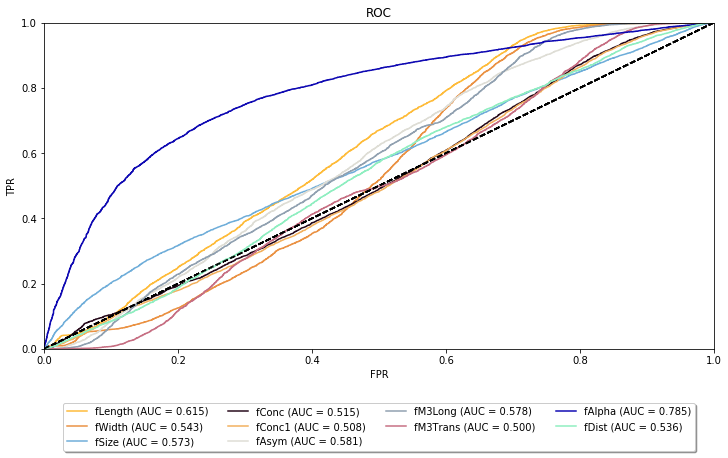
\includegraphics[width = 3in, height=3in]{Univariate_1.png}} &
\subfloat[Correlation Matrix]{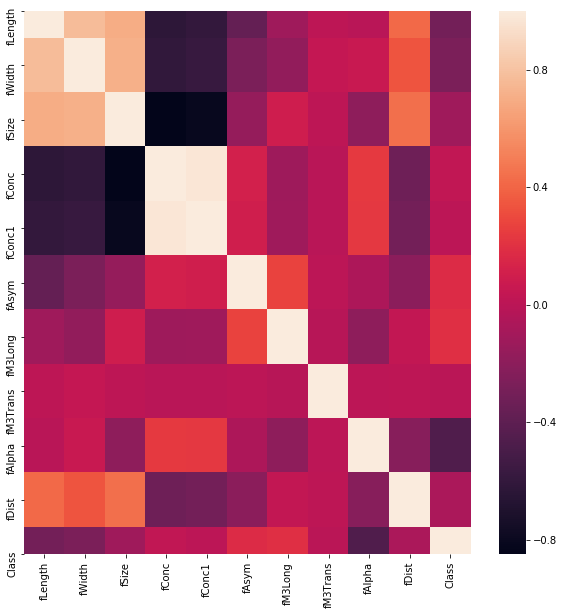
\includegraphics[width = 3in]{CorrMat_1.png}} \\
\end{tabular}
\caption{Feature Correlation}
\end{figure}

The only extrapolations we make from the charts above are that our feature {\tt fAlpha} has a much larger ROC than the rest of the features and that {\tt fConc} and {\tt fConc1} are highly (and linearly) correlated. We notice that our ratio of positive events to negative events is about $.65$, so an AUC of about $.78$ could be significant. We find application for this information when feature engineering 

Our next step is to check if any feature or features provide an exceptional amount of mutual information, which we find using a standard decision tree. 

\begin{figure}[!h]
    \centering
    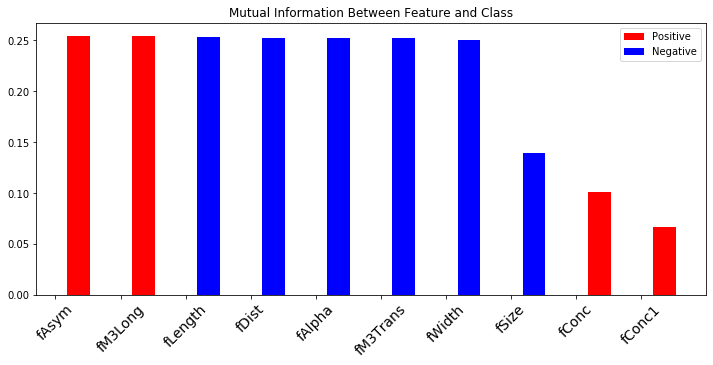
\includegraphics[width = 6in]{MI_1.png} 
    \caption{Mutual Information by Feature}
\end{figure}

We see that no feature stands out and a few are exceptionally unhelpful, namely {\tt fSize} and our correlated features {\tt fConc} and {\tt fConc1} again. Specifically, we see that {\tt fAlpha} is not actually providing any more information than most of the other features, bringing into question if the value of {\tt fAlpha} is actually deducible from our other features. This lessens our optimism for the predictive capabilities of {\tt fAlpha}.

Though there are some insights to be had, overall this feature analysis is unfruitful. This should not be surprising, however, as this is expected of any sufficiently difficult classification problem with a small number of overall features. This encourages us to pursue feature engineering in our next step. 

\subsection{Data/Feature Engineering}

As mentioned, $M$ has a small number of features compared to events (10 features + Class compared to 19020 events). Thus, we can afford to develop new features which we can append to $M$ to create what we define as $M^{F}$ in the hopes that one or more aid in the classification. Before proceeding we first must acknowledge that, for feature engineering, domain knowledge would be very useful. There is of course some link between these features and the event class, but it is almost certainly non-linear. Because of our lack of domain knowledge, we resort to creating non-linear sub-features based off of our existing in hopes that we can catch some of that relationship. We also note that every additional feature is only a function of one other feature (aside from one exception), which is done due to computational limitations. In continuing research, our feature engineering would be more robust and include domain insight as well as multi-feature dependent additions.

To create $M^{F}$, we take the square and cube of each feature aside from {\tt fSize}, {\tt fConc}, {\tt fConc1}, as well as the sum of {\tt fConc} and {\tt fConc1} as an extra feature (our one exception), along with the original $M$. We now see

$$dim \left( M \right) = n \times m, dim \left( M^{F} \right) = n \times m^* = 26$$

Another characteristic of $M$ is the ratio of positive and negative events. In $M$, there are $12332 \gamma$ events and $6688 h$, so we upsample the $h$ events and input them into our new dataset defined $M^{U}$. Note that $M^{U}$ has the same amount of features as $M$, so

$$dim \left( M^{U} \right) = n^* \times m , n^* = 24664 \left(12332 \gamma, 12332 h\right)$$

The hope is that the extra negative events encourage our models to put more weight on the possibility of negative, implying more certainty when guessing positive events, improving our precision. 

After building these datasets, we perform a similar feature analysis as was originally performed on $M$ to the features of $M^{F}$ not already in $M$. We found that no feature developed had any greater feature importance or AUC.  Note that $M^{U}$ would perform identically across all of our metrics, as we have only changed the event distribution. 

\section{Modeling \& Evaluation}

\subsection{Methods}

So far, we have gained no insight into how we would build a classifier for this problem using standard feature analysis. As such, we resort to testing multiple models in efforts to find progress or patterns in the responses from the data. Before doing this, however, we must define how we will be evaluating our models, to know what progress would look like. Firstly, we note that we are using a testing size of $25\%$, and will for all training/testing splits (this does not apply to cross validation). Secondly, we set our predefined value $t=.8$, which is a threshold mentioned in \cite{CaseStudy}. We also explore results with $t=.9$, but we go on to find that our performance is too poor to maintain that level of certainty. This is further elaborated on in deployment. We also note that all models are trained/tested on a normalized variant of our datasets $M, M^{F}, M^{U}$. This is done for consistency and performance, as well as to ensure compatibility when we move on to our stacked voter. With this, we can outline our process. 

We go on to build what we call our "Baseline Models", to get an understanding for how well a generic classifier is performing. After gathering some insight from our baselines, we go on to tune the parameters for a select number of models using stratified cross validation, performing this process across each of our 3 datasets which we will call $\bar{M} = \left\{ M, M^{F}, M^{U} \right\}$. It is important that we stratify since we look to examine how the ratio of positive and negative events in a dataset might impact model performance.  We then evaluate the performance of our tuned models, showing only the results of the models whose baselines were above average. 

Finally, we build a stacked ensemble voting model, combining our three tuned models in an effort to improve our AUC. We attempt to see if different classifiers are correctly assessing different events such that a voter model would have increased event coverage. If we see a degradation in performance, we could also assess if a single model is performing exceptionally poorly and is essentially only correctly identifying a subset of a more robust model. This exploration yields less fruitful than we had hoped, but is rather efficient in its classification thus there is room for improvements and increases in complexity, and acts as another proxy for evaluating model performance. 


\subsection{Baseline Models}

The models we set baselines for are the following:

\begin{itemize}
	\item Decision Tree ($DT$)
	\item Logistic Regression ($LR$)
	\item Random Forest ($RF$)
	\item SVM Linear Kernel ($SVM_L$)
	\item SVM Polynomial Kernel* ($SVM_P$)
	\item Random Forest with Bagging* ($RF_B$)
\end{itemize}

Models marked with an asterisk (*) signify that these were added to the baseline model list after initial testing. We noticed that on our initial training, $SVM_L$ took very long to run and performed very poorly, while $RF$ stood out in AUC. It is discussed in \cite{CaseStudy} that event classification is correlated with the energy level of air shower. This is not information we directly know, but we assert that if there is some non-linear relationship between the energy level of the air shower and our data, if we used models more capable of approximating a non-linear relationship, we should find better classification performance. We thus include other models that have shown to approximate or overcome non-linear relationships well.

We also note that at this point, we have 3 isolated datasets. Therefore, we must train and set a baseline on each to see if our changes will help performance. This isn't too much of a challenge at the stage of setting baselines, but becomes a factor when we move on to hyper-parameter tuning. Baseline Tables and Charts are located in the appendix.

\subsection{Model Tuning}

After setting our baselines, we move on to model tuning. The main challenge we faced in our model tuning is performance. Some models are simply more computationally expensive than others, and thus training across a big search space of parameters is anywhere from impractical to impossible. Thus, we make some choices to moderate the computational complexity we will face. 

First, we limit any cross-validation to 3 stratified data folds. We acknowledge that 3 folds leaves a large proportion of events in testing, but this allowed us to test more parameters as well as have some confidence in the testing. Since these validations occur "behind the scenes" of the code, (that is, we do not see how each subset of parameters perform), a large testing set has benefits. Further more, we chose models which not only performed relatively well in our baselines, but also ran particularly quickly. As such, we chose out $DT, LR$ and $RF$. We would have liked to analyze $SVM_P$ and $RF_B$ instead of $LR$ and $RF$, but they performed too poorly especially on $M^{F}$. Below are the parameters we tune for each model with the corresponding values

\begin{itemize}
	\item Decision Tree ($DT$)
    	\begin{itemize}
    	\item max depth of tree | [10, 22, 35, 47, 60, 72, 85, 97, 110, None]
    	\item Number of features to consider | All, $\sqrt{n}$
    	\item minimum samples per leaf | [25, 40, 60, 90, 120, 175]
    	\item minimum samples to split | [25, 40, 60, 90, 120, 200]
    	\end{itemize}
	\item Logistic Regression ($LR$)
	    \begin{itemize}
    	\item C (regularization term) | [.0001, .001, .005, .01, .05, .1, 1, 10, 20]
    	\item Penalty | L1, L2
    	\item Solver | {\tt liblinear, saga}
    	\end{itemize}
	\item Random Forest ($RF$)
	    \begin{itemize}
    	\item $DT$ List
    	\item number of trees in forest | [25, 64, 103, 142, 182, 221, 260, 300]
    	\item Bootstrap sampling (binary) | {\tt True, False}
    	\end{itemize}
\end{itemize}

We also must note that for $DT$ and $LR$, their training speed allowed us to perform a grid search on the subspace of possible parameter values, thus we tested all possible combinations of values from the predetermined sets of value. This is not true for $RF$ however which, due to the longer training time and larger number of hyper-parameters, necessitated we use a random search across the subspace. 

Located in the appendix is the performance of the tuned models with what we found to be the optimal hyper-parameters. We show the performance of $DT, LR$ and $RF$ on the standard scaled data, for comparison to our voter.

\subsection{Voter}

After tuning our models, we admit that we see only marginal gains in performance, specifically our AUC, if that. We also notice that almost any attempt to improve a model's precision at this stage comes at the cost of it's recall. This dissuades us from further tuning models and instead look to how we could combine their results in the hopes of improving overall classification. 

There is reasonable motivation behind this decision. We mentioned earlier that our baselines for $t=.9$ were quite poor, and thus we didn't follow through developing under this constraint. What we noticed more specifically, is that the incremental precision improvements we saw by increasing our threshold came at the cost of a large amount of precision. 

This led us to speculate that there is perhaps a subset of $\gamma$ events which are particularly difficult to classify, and thus increasing our threshold would force our model to incorrectly predict $h$ for most of the members of this subset. We have exhausted attempts at improving a single model's performance such that it will classify this subset as $\gamma$ with the demanded confidence.  An alternative is to evaluate if different models are performing differently within this subset. We can say that, if there are difference in the evaluation of events in this subset across models, taking a hard voting across said models should improve our overall classification without cost on recall we pay by increasing our threshold. That is, if all 3 models are in agreement or disagreement (which should be the majority of events), the classifications of our voter will be the same. However, if a model disagrees with the other two (in either direction), we can override that classification through hard voting. Unless there is a standout algorithm, performing exceptionally well in this challenging area (which we highly doubt), the overall performance should improve in these edge case. We acknowledge that expectations of drastic metric improvement isn't warranted, but we do expect some metric improvement at little to no cost in recall. 

This leads us to our stacking voting system, where we combine our 3 tuned models into a single classifier. The performance of our final stacked voting classifier is below.

\begin{center}
\begin{tabular}{|p{3cm}||p{2cm}|p{2cm}|p{2cm}|p{2cm}|}
 \hline
 \multicolumn{5}{|c|}{Metrics for Tuned Models} \\
 \hline
 Model | Metric & AUC  & Precision & Recall & Accuracy  \\
 \hline
 Voter  & .83 & .86 & .94 & .86 \\
 \hline
\end{tabular}
\end{center}

\begin{figure}[!h]
    \centering
    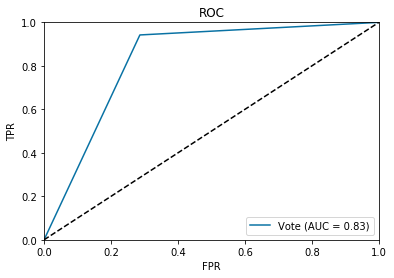
\includegraphics[width = 4in]{Voter.png} 
    \caption{Stacked Voter ROC Curve}
\end{figure}


\section{Deployment}

When discussing deployment, we must immediately acknowledge that the performance of our model(s) do not satisfy the requirements of the use case.

In reality $\gamma$ events are much rarer than in $M$, thus there is a nontrivial cost to classifying a $\gamma$ event as noise, our false negative. In our models, we compensate for the more costly case of a false positive with $t$, but some improvements do come at the cost of more false positives. This could lead to wasting resources by overlooking events that should be investigated further. 

There are some conclusions that we can draw. \cite{CaseStudy} discusses the existence of a limit (Bayesian limit) to the separability the algorithms tested could achieve. Thus we don't project ground-based telescopes absorbing the task of $\gamma$-ray observation completely. However, we found that certain algorithms can outperform others, as well as certain algorithms finding progress with different datasets. Particularly, we found that by using a stacked voting classifier, we could find a balanced model with and improved precision, which was a target metric. Given more models and more robust tuning, more progress should be possible. Finally, the computational bottleneck we reached indicates that more time is needed in the area of optimization, as well as possible improvements in hardware. 

%----------------------------------------------------------------------------------------
%	BIBLIOGRAPHY
%----------------------------------------------------------------------------------------
\newpage
\printbibliography[title={Bibliography}] % Print the bibliography, section title in curly brackets

%----------------------------------------------------------------------------------------

\newpage
\section*{Appendix}
\subsection*{Pairplot}
\centering
\begin{figure}[h]
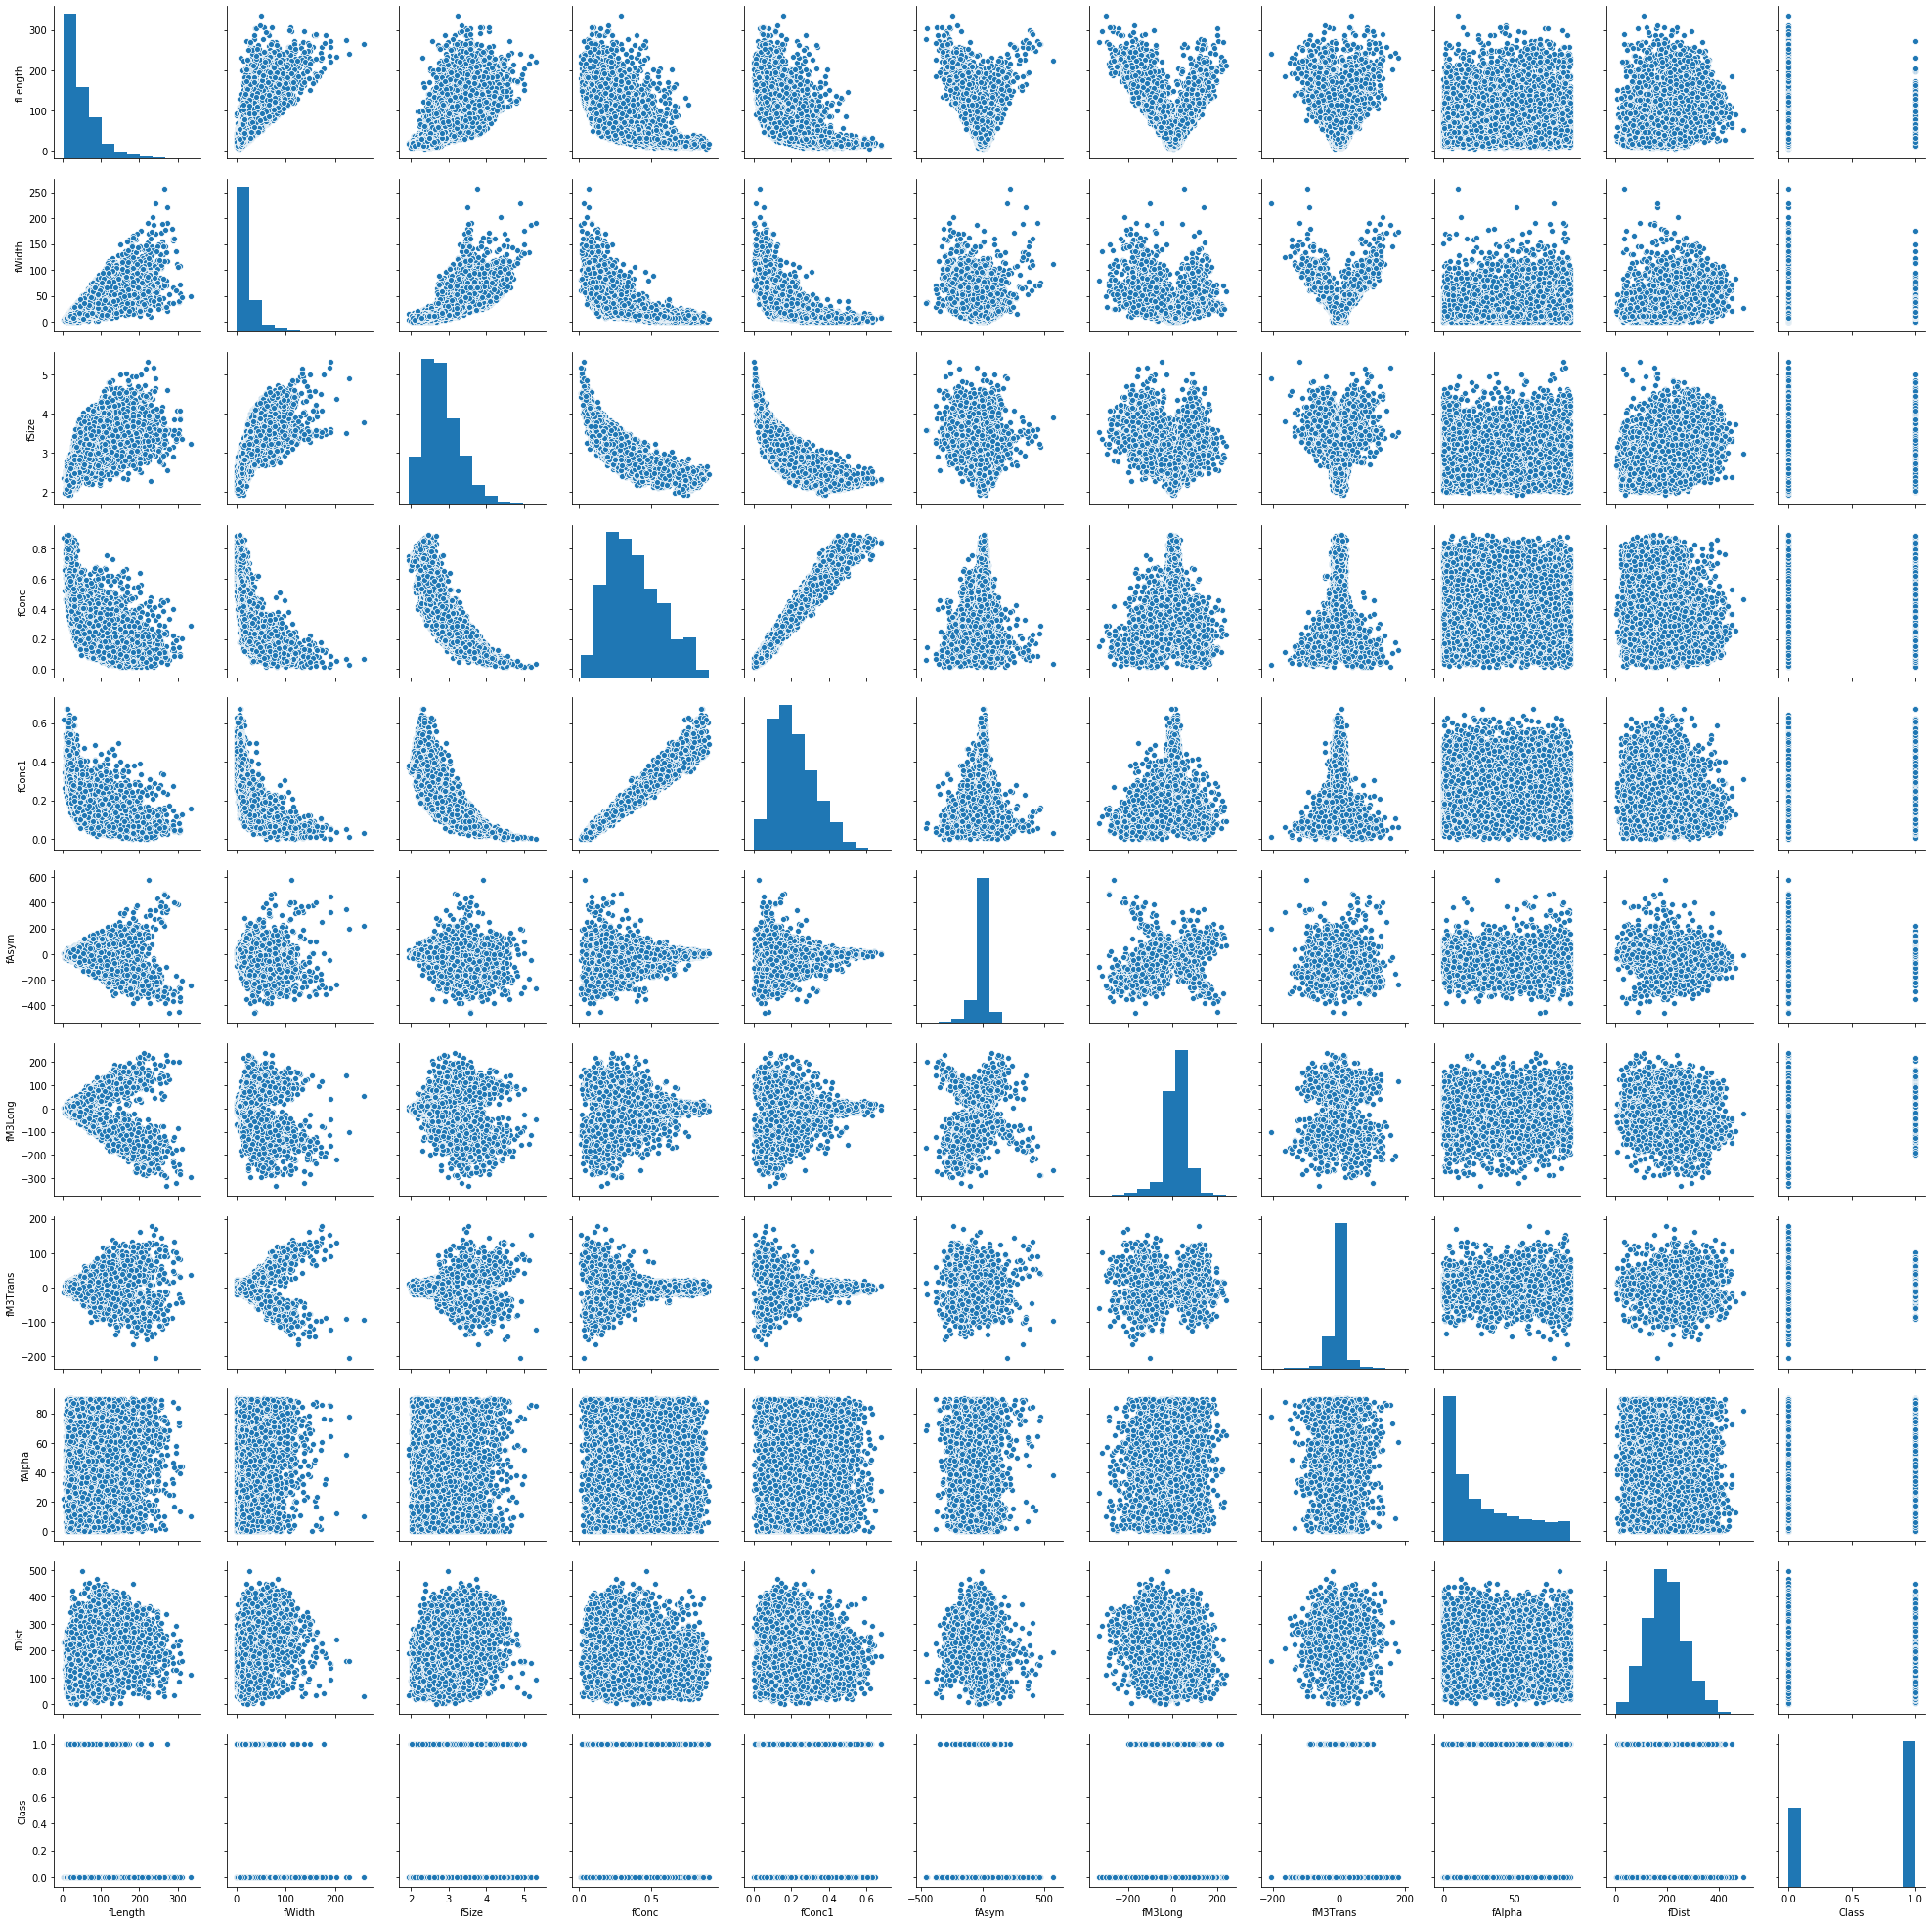
\includegraphics[width = 7in]{pairplot.png} 
\caption{Feature PairPlot}
\end{figure}


\newpage
\subsection*{Baseline}

\begin{figure}[!h]
\centering
\begin{tabular}{ccc}
\subfloat[Decision Tree]{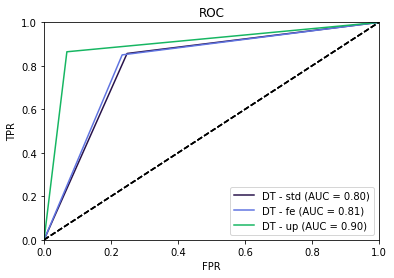
\includegraphics[width = 3in]{DT.png}} &
\subfloat[Random Forest]{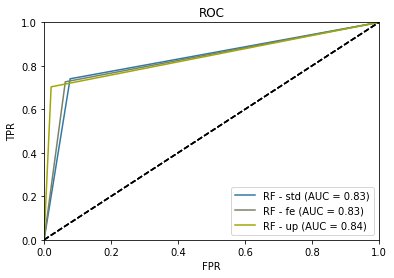
\includegraphics[width = 3in]{RF.png}} \\
\subfloat[RF with Bagging]{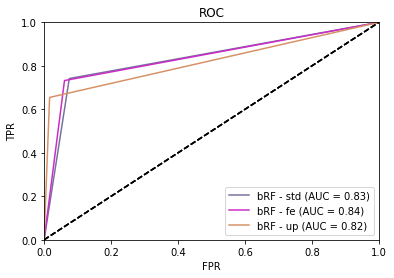
\includegraphics[width = 3in]{bRF.png}} &
\subfloat[LogReg]{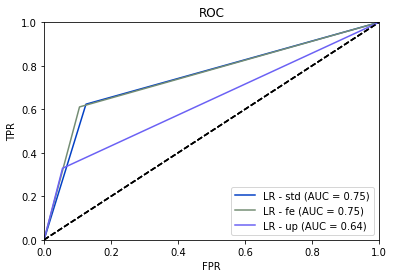
\includegraphics[width = 3in]{LR.png}} \\
\subfloat[SVM Linear]{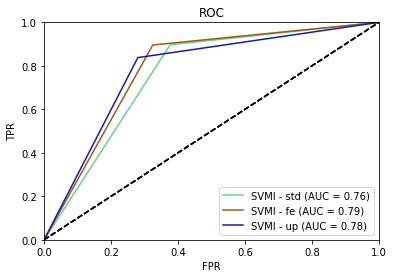
\includegraphics[width = 3in]{SVM_l.png}} &
\subfloat[SVM Poly]{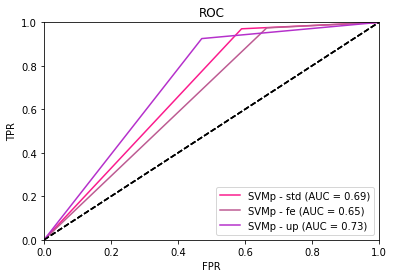
\includegraphics[width = 3in]{SVM_p.png}}\\
\end{tabular}
\caption{Baseline ROC Curves}
\end{figure}


\newpage

\begin{tabular}{ |p{3cm}||p{2cm}|p{2cm}|p{2cm}|p{2cm}|}
 \hline
 \multicolumn{5}{|c|}{Baselines for $M$} \\
 \hline
 Model | Metric & AUC  & Precision & Recall & Accuracy  \\
 \hline
 $DT$  & .80 & .87 & .86 & .82 \\
 $RF$  & .83 & .95 & .74 & .80 \\
 $RF_B$   & .83 & .95 & .74  & .81 \\
 $LR$   & .75 & .90 & .62 & .71 \\
 $SVM_L$  & .76 & .82 & .90 & .80 \\
 $SVM_P$  & .69 & .76 & .97 & .78 \\
 \hline
\end{tabular}

\begin{tabular}{ |p{3cm}||p{2cm}|p{2cm}|p{2cm}|p{2cm}|}
 \hline
 \multicolumn{5}{|c|}{Baselines for $M^{F}$} \\
 \hline
 Model | Metric & AUC  & Precision & Recall & Accuracy  \\
 \hline
 $DT$  & .81 & .87 & .85 & .82 \\
 $RF$  & .83 & .95 & .73 & .80\\
 $RF_B$   & .84 & .96 & .83 & .71 \\
 $LR$   & .75 & .91 & .61 & .71 \\
 $SVM_L$  & .79 & .84 & .90 & .82\\
 $SVM_P$  & .65 & .73 & .97 & .85 \\
 \hline
\end{tabular}

\begin{tabular}{ |p{3cm}||p{2cm}|p{2cm}|p{2cm}|p{2cm}|}
 \hline
 \multicolumn{5}{|c|}{Baselines for $M^{U}$} \\
 \hline
 Model | Metric & AUC  & Precision & Recall & Accuracy  \\
 \hline
 $DT$  & .90 & .93 & .86 & .90 \\
 $RF$  & .84 & .97 & .70 & .84 \\
 $RF_B$   & .82 & .98 & .65 & .82 \\
 $LR$   & .64 & .86 & .33 & .64 \\
 $SVM_L$  & .78 & .75 & .84 & .78 \\
 $SVM_P$  & .73 & .66 & .93 & .73 \\
 \hline
\end{tabular}


\newpage
\subsection*{Tuned Models}

\begin{tabular}{|p{3cm}||p{2cm}|p{2cm}|p{2cm}|p{2cm}|}
 \hline
 \multicolumn{5}{|c|}{Metrics for Tuned Models} \\
 \hline
 Model | Metric & AUC  & Precision & Recall & Accuracy  \\
 \hline
 $DT$  & .80 & .91 & .65 & .75 \\
 $RF$  & .83 & .90 & .76 & .84 \\
 $LR$   & .75 & .90 & .62 & .71 \\
 \hline
\end{tabular}

\begin{figure}[h]
\centering
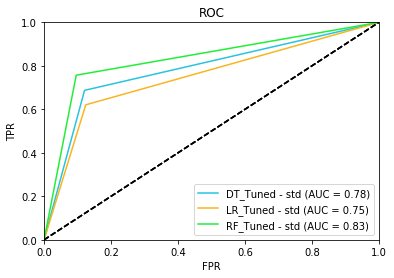
\includegraphics[width = 5in]{DTLRRF.png} 
\caption{Tuned ROC Curves}
\end{figure}


\end{document}
